\section{Neural Network Model}

Since this problem is to classify images, we chose to use a deep neural network to efficiently and accurately solve the problem.
Specifically, we were using a convolutional neural network to detect whether people in the images were wearing masks.

\subsection{Model Structure}

The model receives a batch of grayscale images with the size of 128 pixels by 128 pixels as an input.
In order to predict the output, the model makes use of several hidden layers to come up with probability distribution (or predictions).

The model consists of three convolutional layers with a max-pooling layer after each of them.
We performed a batch normalization at the last convolutional neural network to make the model learns better. 
Moreover, we flattened the last max-pooling layer out to input into two fully connected layers which eventually predicted the output of the model.
The model can classify images into two classes–with mask and without mask. See Figure~\ref{fig:model-structure}.

\begin{figure}
  \caption{
    the architecture of the convolutional neural network,
    which consists of three convolutional layers with a max-pooling layer after each of them.
    The output from the last layer then being inputted into the last two fully connected layers which predict the final output.
  }
  \label{fig:model-structure}
  \centering
  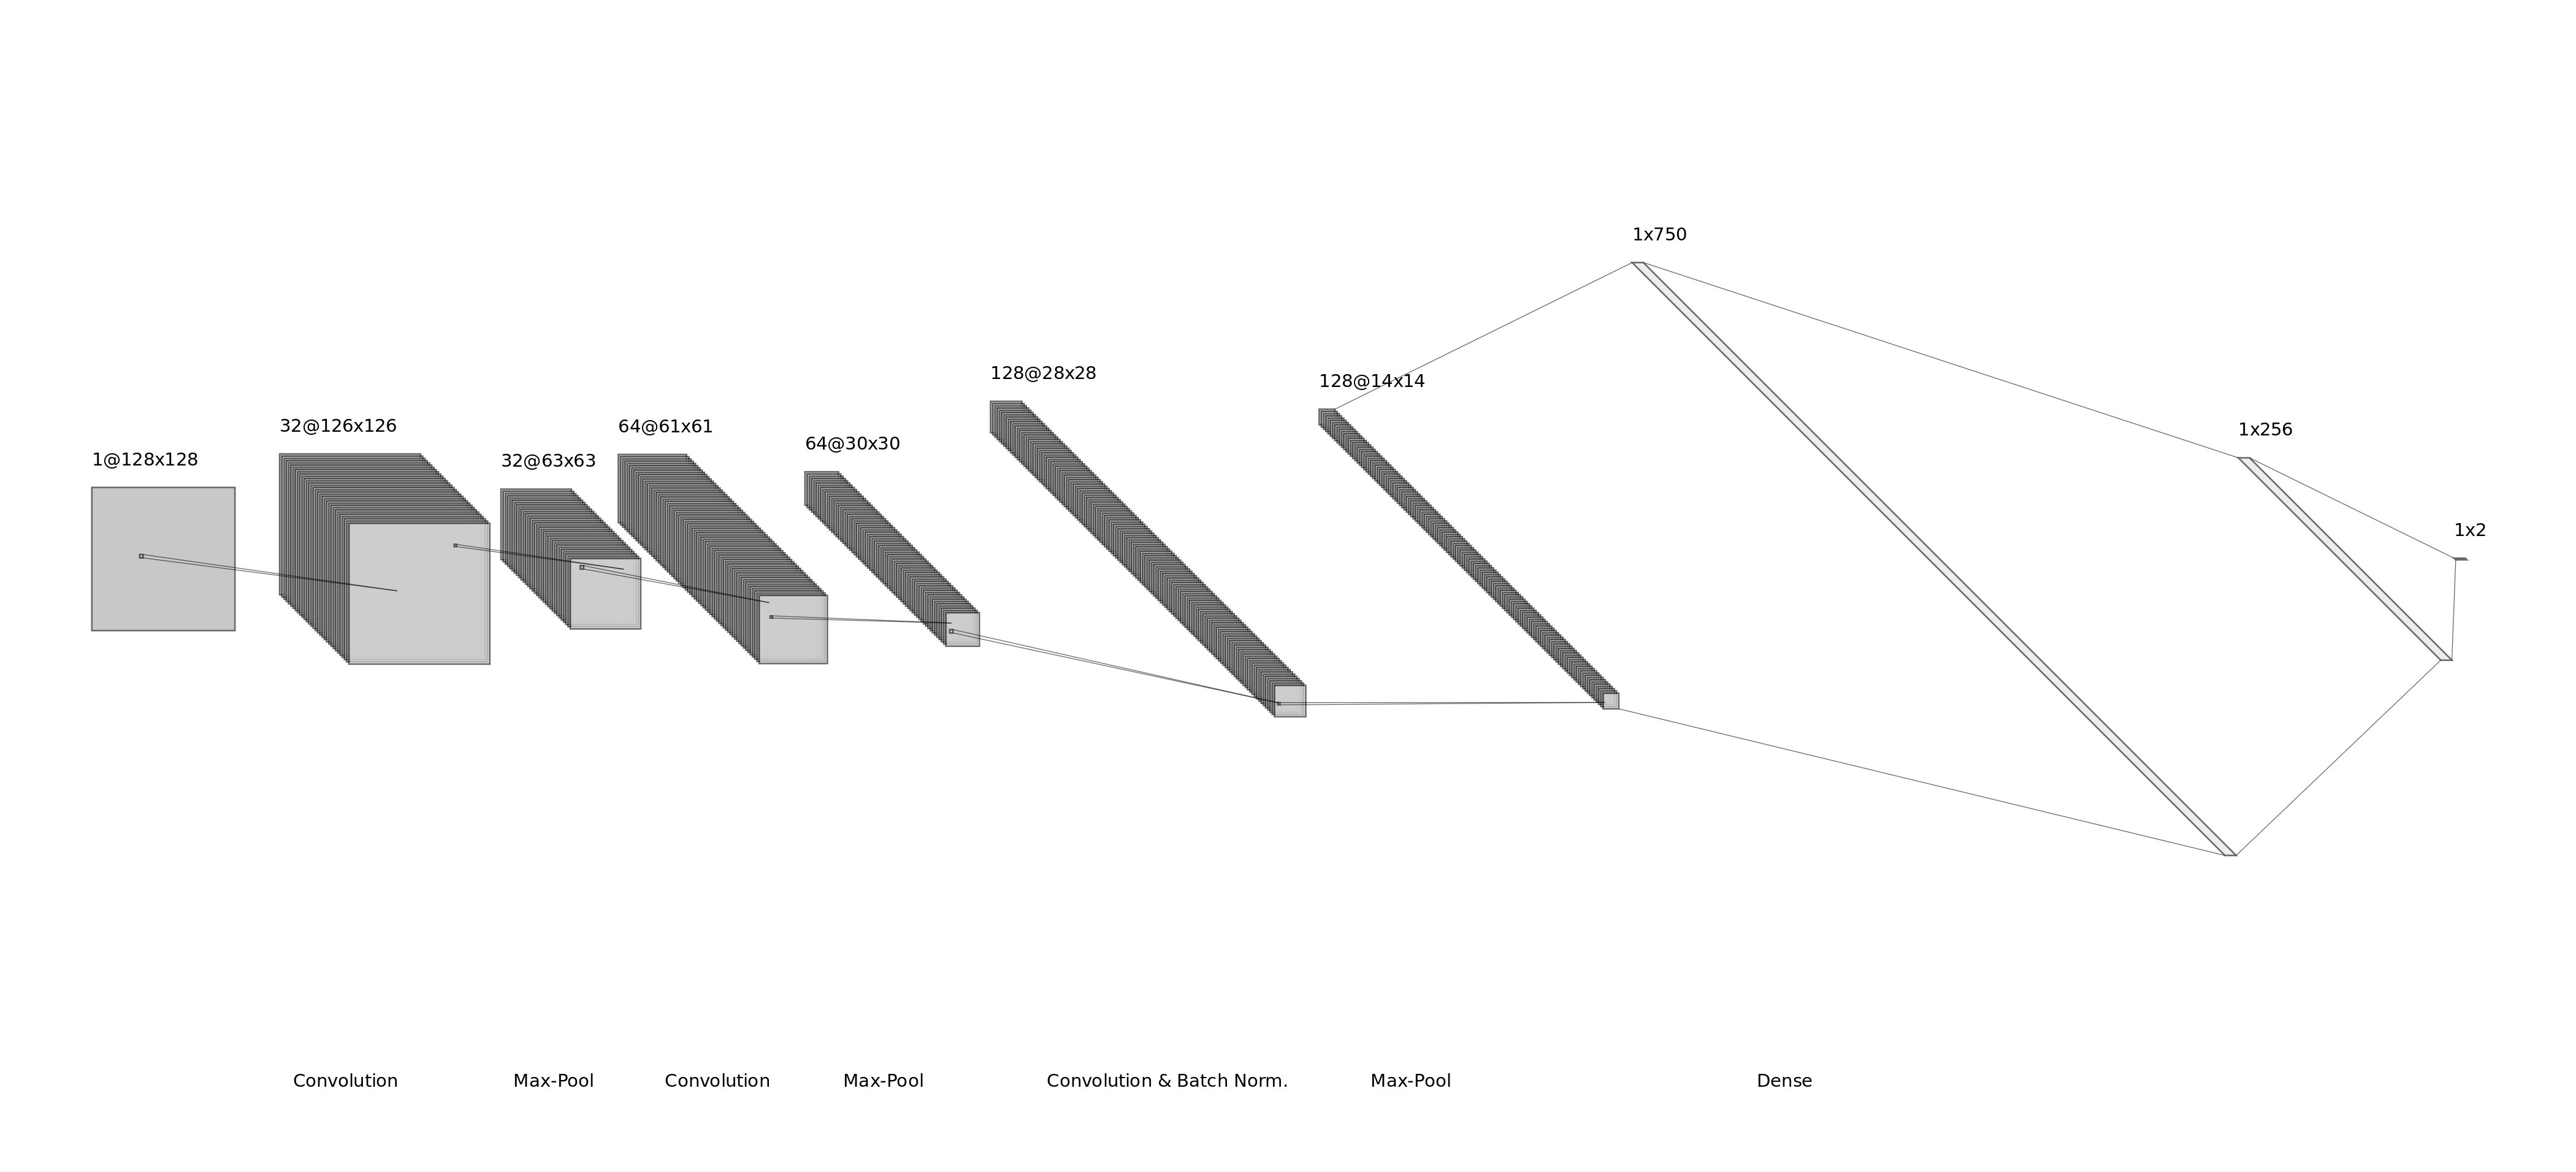
\includegraphics[width=400px]{figures/model-structure.jpg}
\end{figure}


\subsection{Loss Function and Optimizer}

We used softmax and cross-entropy as our loss functions.
We used softmax at the end of our prediction because the softmax function simulated the probability of an input image being one of the two classes.
And, we used the cross-entropy function at the end because we would like to amplify the loss value to penalize the model when it predicted incorrectly.
For an optimizer for our training, we used SGD because a model trained with SGD is less likely to overfit the dataset as it chooses data points at random.
